\documentclass{article}

% if you need to pass options to natbib, use, e.g.:
 \PassOptionsToPackage{numbers, compress}{natbib}
% before loading nips_2018

% ready for submission
%\usepackage{nips_2018}

% to compile a preprint version, e.g., for submission to arXiv, add
% add the [preprint] option:
% \usepackage[preprint]{nips_2018}

% to compile a camera-ready version, add the [final] option, e.g.:
 \usepackage[final]{nips_2018}

% to avoid loading the natbib package, add option nonatbib:
% \usepackage[nonatbib]{nips_2018}

\usepackage[utf8]{inputenc} % allow utf-8 input
\usepackage[T1]{fontenc}    % use 8-bit T1 fonts
\usepackage{hyperref}       % hyperlinks
\usepackage{url}            % simple URL typesetting
\usepackage{booktabs}       % professional-quality tables
\usepackage{amsfonts}       % blackboard math symbols
\usepackage{nicefrac}       % compact symbols for 1/2, etc.
\usepackage{microtype}      % microtypography
\usepackage{comment}

%%%%%%%%%%%%%%%%
%%%%%My Packages%%%%%
%%%%%%%%%%%%%%%%

\usepackage{amsmath, amssymb, amsthm, mathtools}

\newtheorem{theorem}{Theorem}[section]
\newtheorem{definition}{Definition}[section]

\usepackage{enumerate,xcolor}
\usepackage{tikz,hyperref}
\usetikzlibrary{spy,calc,patterns,arrows,decorations.pathmorphing,backgrounds,positioning,fit,petri,mindmap,trees,intersections}
\usepackage{algorithm}
\usepackage{algorithmic}
\usepackage{bm}

\def\CC{{C\nolinebreak[4]\hspace{-.05em}\raisebox{.4ex}{\tiny\bf ++}}}



\newcommand\DoubleLine[7][1pt]{%
    \path(#2)--(#3)coordinate[at start](h1)coordinate[at end](h2);
    \draw[#4]($(h1)!#1!90:(h2)$)-- node [left=-.75mm] {#5} ($(h2)!#1!-90:(h1)$); 
    \draw[#6]($(h1)!#1!-90:(h2)$)-- node [right=-.75mm] {#7} ($(h2)!#1!90:(h1)$);
    }


\newcommand\note[1]{\textcolor{blue}{#1}}

%\usepackage[lining]{sourcesanspro}



\title{Game Theoretical Approaches in \\ Multi-Agent Reinforcement Learning}

% The \author macro works with any number of authors. There are two
% commands used to separate the names and addresses of multiple
% authors: \And and \AND.
%
% Using \And between authors leaves it to LaTeX to determine where to
% break the lines. Using \AND forces a line break at that point. So,
% if LaTeX puts 3 of 4 authors names on the first line, and the last
% on the second line, try using \AND instead of \And before the third
% author name.

\author{
Sai Ganesh Nagarajan\footnote{equal contribution}\\
Student ID: 1003206
  %% examples of more authors
\And
Jin Xing Lim$^\ast$ \\
Student ID: 1003964  %% \AND
  %% Coauthor \\
  %% Affiliation \\
  %% Address \\
  %% \texttt{email} \\
  %% \And
  %% Coauthor \\
  %% Affiliation \\
  %% Address \\
  %% \texttt{email} \\
  %% \And
  %% Coauthor \\
  %% Affiliation \\
  %% Address \\
  %% \texttt{email} \\
}

\begin{document}
% \nipsfinalcopy is no longer used

\maketitle

\section{Introduction}
We study the game theoretical problems that arise in multi-agent learning. In particular, we are interested in the simplest possible setting of symmetric zero-sum games,i.e, games that look like rock-paper-scissors, in the sense that there is no dominant agent/strategy. A recent paper that tries to address this problem \cite{Balduzzi2019OpenendedLI}, talks about a variant of previously proposed multi-agent reinforcement learning algorithm \cite{NIPS2017_7007} called the Policy Space Response Oracles (PSRO), where they showed improved performance compared to learning independent reinforcement algorithm. We will look at these two algorithms and interpret the game theoretical intuition behind them. In addition, we re-created some experiments in \cite{Balduzzi2019OpenendedLI} to understand the working of the algorithms.

\section{Policy Space Response Oracles}
In this section, we describe the fundamental multi-agent learning algorithm (Figure \ref{fig:psro_marl}), first described in \cite{NIPS2017_7007}, based on which more recent developments have been made for the symmetric zero-sum case, which discusses variants of PSRO.

\begin{figure*}[!ht]
	\centering
	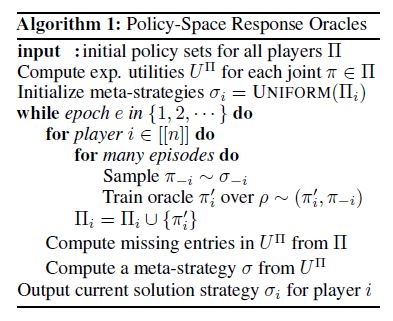
\includegraphics[scale=0.6]{PSRO_marl}
	%  \fbox{\rule[-.5cm]{0cm}{4cm} \rule[-.5cm]{4cm}{0cm}}
	\caption{\textit{$PSRO$ Algorithm}}
	\label{fig:psro_marl}
\end{figure*}

The main intuition of the algorithm arises from how we analyze games in general, when analyzing the strategies taken by agent $i$, we fix the other agents' strategies and see the effect on the payoff to agent $i$, if $i$ changes his/her strategy. 

The high-level description of the algorithm is as follows:
\begin{enumerate}
	\item Initially all agents have their own initial policies and say they have an uniform probability distribution over these initial policies.
	\item Next, an empirical game matrix is calculated by computing the expected payoffs that each agent would get for using policy $\pi_i$. Enumerate the matrix with all possible combinations of the policies that each agent can take.
	\item Given agent $i$ and fixing all the agents stochastic policies, i.e, using the current probability distribution over their policies (also referred to as meta strategies), agent $i$ then learns a ``best response'' using an oracle, which may be a standard single agent reinforcement learning algorithm, or as simple as a function that implements gradient descent.
	\item Once all the agents repeat the above step, these policies are added to the empirical game matrix and the remaining entries are filled.
	\item Finally, the agents update their meta strategies over their "deterministic" policies based on the empirical payoff matrix and using an update rule such as MWU, or RD or PRD (to encourage exploration).
\end{enumerate}

The nature of the algorithm is to decouple the game theory aspect (obtaining the meta strategies using an update rule) and the reinforcement learning aspect, which goes into the oracle and helps us obtain a best response policy when fixing the others. This allows to study them separately. In addition, the algorithm's limit behavior depends on the nature of the empirical game and the update rule being used. We know that most of the discrete time update rules for high dimensional games are chaotic and diverging \cite{bailey2018multiplicative}. Even in continuous time, the dynamics are known to be recurrent for zero-sum games \cite{mertikopoulos2018cycles}. This in itself raises many interesting questions with regards to training of the agents in these settings.
Since, the general case is complex, we will try to analyze a much simpler setting and look at the problem of training agents when playing a symmetric zero-sum game. The main question is how do we aim to get ``better'' agents while playing a symmetric zero-sum game, where there is no clear winner (or dominant agent).
\section{Towards Population Objectives in Zero-Sum Games}
The main argument in \cite{Balduzzi2019OpenendedLI}, is that in the case when agents are playing a symmetric zero-sum game, where there is no one best agent, one way to train is by diversifying the strategies that the agents play, by trying to discover new strategies. So this requires maintaining a population of agents and improving this population over time, as opposed to self-play where the best agent trains against itself and improves over time. The paper argues that self-play is not effective in games where there is no best agent and hence defines certain classes of games that can be studied by keeping this in mind.
\subsection{Zero-sum Games: Transitive + Cyclic}
The main idea is that, there are some games that are transitive meaning, any local improvements will eventually lead to global optimum. We can imagine these games to have ``gradient-line'' behavior. These are the class of games where self-play may suffice, for instance, Chess, Go, Laser-tag etc.
There are other games which are cyclic, in the sense that there is no best agent. These are the games that look like rock-paper-scissors. For instance, more complex games such as DOTA, Starcraft may exhibit this type of behavior where you require different skills in a team and diversification to win matches.
\subsection{Training Objectives}
We establish some notations to talk about the algorithm. Consider $v,w \in \mathcal{W}$, where $v,w$ maybe weights of a neural net. We will henceforth refer to them as agents. The agents are chosen from the space of agents $\mathcal{W}$. We define $\phi(v,w)$ to be the expectation of $v$ winning against $w$ and according to this definition we have $\phi(v,w)=-\phi(w,v)$, since it is a symmetric zero-sum game. We can then define a population of agents $\beta=\{v_1,v_2,\ldots,v_K\}$, where this population contains $K$ agents. 
Now, we can populate the empirical game matrix (or evaluation matrix $A_{\beta}$) as the payoff matrix when population $\beta$ competes with itself. Formally, $A_{\beta}^{i,j}=\phi(v_i,v_j)$, where $A_{\beta}^{i,j}$ is the $(i,j)^{th}$ element of $A_{\beta}$.
Finally, with the population at hand, we can look at training agents when, i.e, getting a best response oracle when the other agents in the population plays a Nash mixture which is the notion that has replaced a ``best agent'' in the symmetric zero-sum case and this leads to two algorithms which are modifications of the PSRO for self play in symmetric-zero sum games. For illustration, we look at one algorithm called PSRO -rectified Nash ($PSRO_{rN}$), which is explained in the next section. Also, the Nash equilibrium for this game can be computed via a simple linear program (which however, grows with the number of agents in the population). 
\subsection{Comparison between Self-play and $PSRO_{rN}$}

Two of the algorithms that were used for comparison in Balduzzi et al paper \cite{Balduzzi2019OpenendedLI} are Self-play and $PSRO_{rN}$.

\begin{figure*}[!ht]
	\centering
	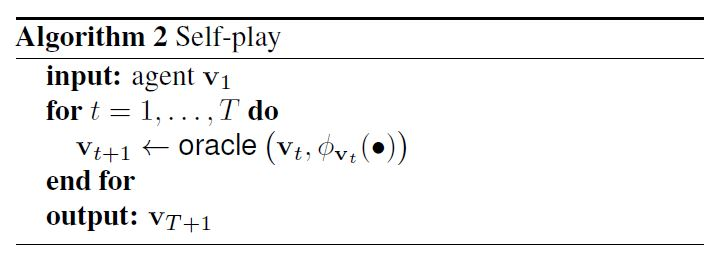
\includegraphics[scale=0.5]{SelfPlay}
	%  \fbox{\rule[-.5cm]{0cm}{4cm} \rule[-.5cm]{4cm}{0cm}}
	\caption{\textit{Self-play Algorithm}}
	\label{fig:sp_algo}
\end{figure*}

For Self-play algorithm (Figure \ref{fig:sp_algo}), it essentially trains the next agent using the current agent via an oracle. This algorithm has been shown to be effective in training agents in games like Chess, Go and other games \cite{silver2018general}. However, Self-play requires the game to be transitive in order for the training to be effective. Training through self-play on cyclic games, such as disc game below, is not effective as success against one agent does not guarantee success against the others. 

\begin{figure*}[!ht]
	\centering
	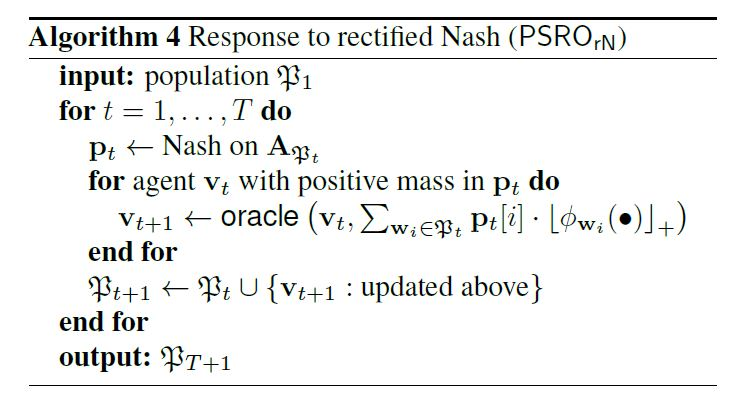
\includegraphics[scale=0.5]{PSRO_rN}
	%  \fbox{\rule[-.5cm]{0cm}{4cm} \rule[-.5cm]{4cm}{0cm}}
	\caption{\textit{$PSRO_{rN}$ Algorithm}}
	\label{fig:psro_algo}
\end{figure*}

As such, the paper introduces another $PSRO_{rN}$ (Figure \ref{fig:psro_algo}) that works well in both transitive and cyclic games. In each iteration, each agent, with support under the Nash equilibrium, is trained against the Nash-weighted mixture of agents that it beats or ties. The idea is to make agents to ``further strengthen on their strengths and ignore their weaknesses''. For transitive games, this algorithm will reduce to classical self-play as the Nash equilibrium would be $(0,...,0,1)$. For cyclic games, this algorithm will generate a more diversified population of strategies to counter different variations of strategies. The intuition behind this is that, the oracle produces an agent that maximizes the convex combination of non-negative functions as shown in the figure. So this ``maximum'' agent has to tie with every other agent or perform better and this has a net effect of improving (or discovering) strategies that perform better and since each significant agent in the population is trained, this leads to a net improvement in the population. 

\section{Experiments}

We ran several experiments to show how the populations from Self-play and $PSRO_{rN}$ algorithms evolved for disc game (cyclic) and transitive version of the lotto game separately.

\subsection{Disc Game \cite{Balduzzi2019OpenendedLI}}

Let $v,w \in \mathbb{R}^2$, where the payoff function is

$$\phi(v,w) = v_1w_2-v_2w_1.$$

Thus, every point in the $\mathbb{R}^2$ is considered as an agent where the value of both coordinates are considered as its strategy. Thus, the payoff of agent $v$ against agent $w$ is measured by $\phi(w,v)$. This game is cyclic (see Figure \ref{fig:disc}, which is taken from Balduzzi et al paper).\\

Note that rock-paper-scissors can be embedded in this disc game via the following transformation: $$r_\epsilon = \frac{\sqrt{3}\epsilon}{2} \big( \cos 0, \sin 0 \big), p_\epsilon = \frac{\sqrt{3}\epsilon}{2} \big(\cos \frac{2\pi}{3}, \sin \frac{2\pi}{3}\big), s_\epsilon = \frac{\sqrt{3}\epsilon}{2} \big(\cos \frac{4\pi}{3}, \sin \frac{4\pi}{3}\big)$$

to obtain the following evaluation matrix:
$$
A_{\{r_\epsilon,p_\epsilon,s_\epsilon\}}= 
\begin{bmatrix} 
0 & \epsilon^2 & - \epsilon^2\\
-\epsilon^2 & 0 & \epsilon^2\\
\epsilon^2 & -\epsilon^2 &0 
\end{bmatrix}
$$

\begin{figure*}[!ht]
	\centering
	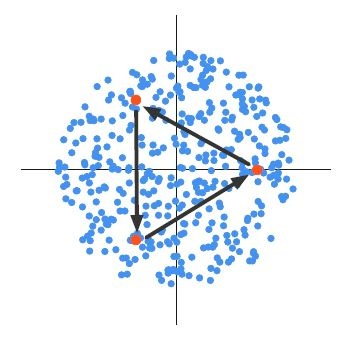
\includegraphics[scale=0.6]{DiscGame.JPG}
	%  \fbox{\rule[-.5cm]{0cm}{4cm} \rule[-.5cm]{4cm}{0cm}}
	\caption{\textit{Disc game}. The points (blue and red) represent a set of strategies from the disc game. The three cyclic strategies' (rock-paper-scissors) relations are shown as red points.}
	\label{fig:disc}
\end{figure*}


We ran Self-play and $PSRO_{rN}$ algorithms with the initial population as $\{r_1,p_1,s_1\}$ (as shown in the transformation above with $\epsilon = 1$). For training under Self-play, the population evolved spirally outwards as shown in Figure \ref{fig:self}. However, as for the population under the $PSRO_{rN}$ algorithm training, the population spread out from each of the initial conditions as shown in Figure \ref{fig:psro}. We can see that population from the $PSRO_{rN}$ algorithm diversified much better than the Self-play algorithm, which only improves the next agent based on the current agent, causing it to move out in a spiral manner.




\begin{figure*}[!ht]
	\begin{minipage}{0.5\linewidth}
		\centering
		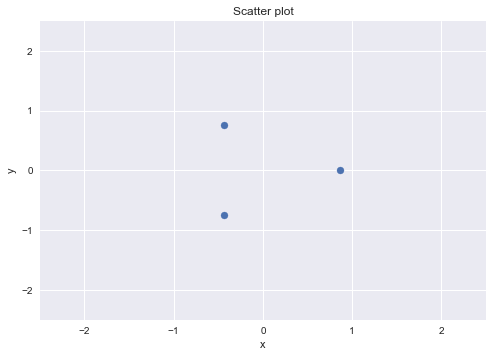
\includegraphics[scale=0.4]{self1}
	\end{minipage}%
	\begin{minipage}{0.5\linewidth}
		\centering
		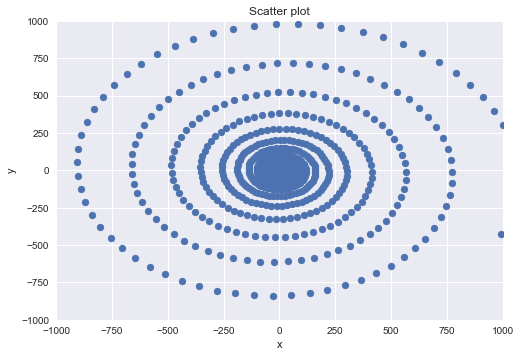
\includegraphics[scale=0.4]{self15}
	\end{minipage}%
	\caption{\textit{Evolution of population through Self-play.} Left: Initial population $\{r_1,p_1,s_1\}$. Right:Final population with size of 1536 (after epochs of training)}
	\label{fig:self}
\end{figure*}

\begin{figure*}[!ht]
	\begin{minipage}{0.5\linewidth}
		\centering
		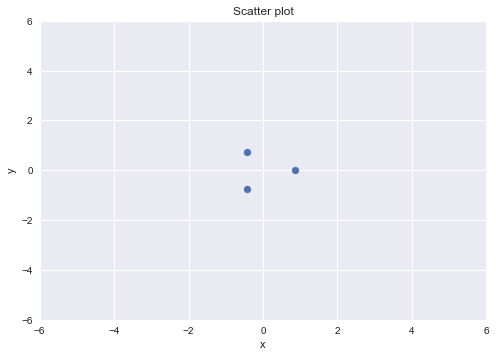
\includegraphics[scale=0.4]{psro1}
	\end{minipage}%
	\begin{minipage}{0.5\linewidth}
		\centering
		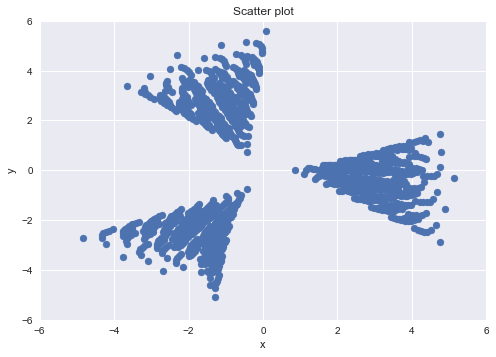
\includegraphics[scale=0.4]{psro16}
	\end{minipage}%
	\caption{\textit{Evolution of population through $PSRO_{rN}$.} Left: Initial population $\{r_1,p_1,s_1\}$. Right:Final population with size of 1536 (after epochs of training)}
	\label{fig:psro}
\end{figure*}

\subsection{Transitive Lotto}

This game is a resource allocation game defined over $[-1,1]^2$ space in the $\mathbb{R}^2$. There is a fixed set $C$ of $n$ customers, $\{c_1,...,c_n\}$, each being a point in the space. Each agent's strategy $(\mathbf{p},\mathbf{v}) = \{(p_1,\mathbf{v_1}),...,(p_k,\mathbf{v_k})\}$, distributes weight $p_i$ over server $\mathbf{v_i} \in [-1,1]^2$ for $1 \leq i \leq k$. The payoff function between two agents, $\mathbf{(p,v)}$ and $\mathbf{(q,w)}$, is defined as

$$\phi(\mathbf{(p,v),(q,w)}) = \sum_{i,j=1}^{c,k}(p_i v_{ij}-q_j w_{ij})$$

where the scalars $v_{ij}$ and $w_{ij}$ depend on the distance between customer $i$ and the servers:

$$(v_{i1},...,w_{ik}) = softmax(\mathbf{-||c_i-v_1||^2,...,-||c_i-w_k||^2}).$$

This game is a transitive version of the lotto game.

We ran Self-play and $PSRO_{rN}$ algorithms for different number of servers ($k=3,9,15$). As mentioned above, we observed that for all cases, the $PSRO_{rN}$ algorithm works the same as Self-play for this transitive lotto game. Regardless of the number of servers ($k=3,9,15$), all servers eventually converge to the centroid of the 9 customers (See Figure \ref{fig:3s}, \ref{fig:9s} and \ref{fig:15s}), which is the best location to serve all customers. As for the probability distribution of the servers, eventually it will converge to uniform distribution.


\begin{figure*}[!ht]
	\begin{minipage}{0.5\linewidth}
		\centering
		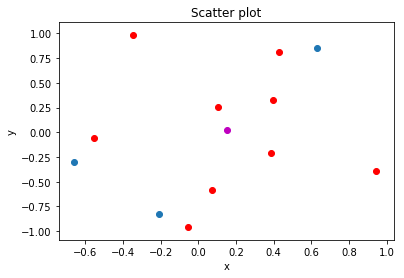
\includegraphics[scale=0.3]{3s0}
	\end{minipage}%
	\begin{minipage}{0.5\linewidth}
		\centering
		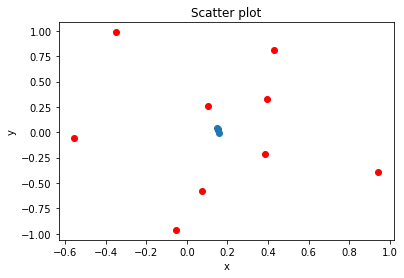
\includegraphics[scale=0.3]{3s10}
	\end{minipage}%
	\caption{\textit{$k=3$ servers.} Right points: Location of 9 customers. Blue points: Location of 3 servers. Magenta point: Centroid of the 9 customers. Left: Initial locations of the servers. Right: Final location of the servers after 100 epoch}
	\label{fig:3s}
\end{figure*}


\begin{figure*}[!ht]
	\begin{minipage}{0.5\linewidth}
		\centering
		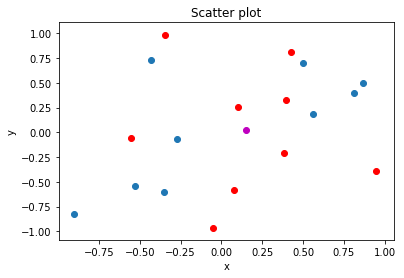
\includegraphics[scale=0.3]{9s0}
	\end{minipage}%
	\begin{minipage}{0.5\linewidth}
		\centering
		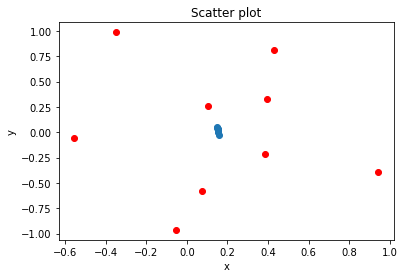
\includegraphics[scale=0.3]{9s10}
	\end{minipage}%
	\caption{\textit{$k=9$ servers.} Right points: Location of 9 customers. Blue points: Location of 9 servers. Magenta point: Centroid of the 9 customers. Left: Initial locations of the servers. Right: Final location of the servers after 100 epoch}
		\label{fig:9s}
	\end{figure*}

\begin{figure*}[!ht]
	\begin{minipage}{0.5\linewidth}
		\centering
		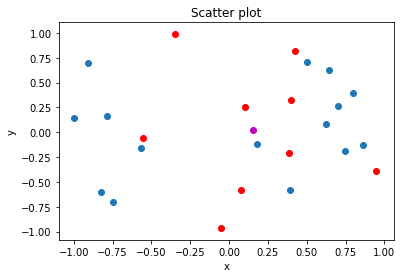
\includegraphics[scale=0.3]{15s0}
	\end{minipage}%
	\begin{minipage}{0.5\linewidth}
		\centering
		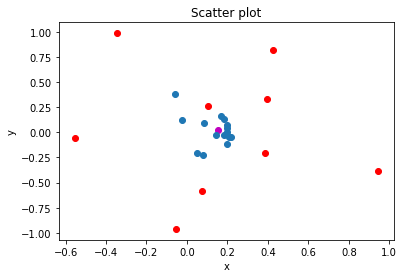
\includegraphics[scale=0.3]{15s10}
	\end{minipage}%
	\caption{\textit{$k=15$ servers.} Right points: Location of 9 customers. Blue points: Location of 15 servers. Magenta point: Centroid of the 9 customers. Left: Initial locations of the servers. Right: Final location of the servers after 100 epoch}
		\label{fig:15s}
	\end{figure*}


\newpage
\section{Future Works}
For future work we can try to extend the idea of self-play to multi-agent settings, via the idea of network (or polymatrix) games, as the understanding of game dynamics \cite{piliouras2014optimization,nagarajan2018three} and the tractability of Nash equilibria \cite{cai2016zero} maybe helpful in achieving effective learning in more complicated multi-agent settings by encoding the interaction through the edges of the network.
\section{Conclusion}
We analyze experimentally and provide intuition to some game theoretical problems surrounding multi-agent learning by looking at some recent learning algorithms.



\bibliographystyle{abbrvnat}
\bibliography{bib}



%%%%%%%%%%%%%%%%%%%%
%%%%%Template Below%%%%%%%
%%%%%%%%%%%%%%%%%%%%

%\newpage
%
%\section{Submission of papers to NIPS 2018}
%
%NIPS requires electronic submissions.  The electronic submission site
%is
%\begin{center}
%  \url{https://cmt.research.microsoft.com/NIPS2018/}
%\end{center}
%
%Please read the instructions below carefully and follow them faithfully.
%
%\subsection{Style}
%
%Papers to be submitted to NIPS 2018 must be prepared according to the
%instructions presented here. Papers may only be up to eight pages
%long, including figures. Additional pages \emph{containing only
%  acknowledgments and/or cited references} are allowed. Papers that
%exceed eight pages of content (ignoring references) will not be
%reviewed, or in any other way considered for presentation at the
%conference.
%
%The margins in 2018 are the same as since 2007, which allow for
%$\sim$$15\%$ more words in the paper compared to earlier years.
%
%Authors are required to use the NIPS \LaTeX{} style files obtainable
%at the NIPS website as indicated below. Please make sure you use the
%current files and not previous versions. Tweaking the style files may
%be grounds for rejection.
%
%\subsection{Retrieval of style files}
%
%The style files for NIPS and other conference information are
%available on the World Wide Web at
%\begin{center}
%  \url{http://www.nips.cc/}
%\end{center}
%The file \verb+nips_2018.pdf+ contains these instructions and
%illustrates the various formatting requirements your NIPS paper must
%satisfy.
%
%The only supported style file for NIPS 2018 is \verb+nips_2018.sty+,
%rewritten for \LaTeXe{}.  \textbf{Previous style files for \LaTeX{}
%  2.09, Microsoft Word, and RTF are no longer supported!}
%
%The \LaTeX{} style file contains three optional arguments: \verb+final+,
%which creates a camera-ready copy, \verb+preprint+, which creates a
%preprint for submission to, e.g., arXiv, and \verb+nonatbib+, which will
%not load the \verb+natbib+ package for you in case of package clash.
%
%\paragraph{New preprint option for 2018}
%If you wish to post a preprint of your work online, e.g., on arXiv,
%using the NIPS style, please use the \verb+preprint+ option. This will
%create a nonanonymized version of your work with the text
%``Preprint. Work in progress.''  in the footer. This version may be
%distributed as you see fit. Please \textbf{do not} use the
%\verb+final+ option, which should \textbf{only} be used for papers
%accepted to NIPS.
%
%At submission time, please omit the \verb+final+ and \verb+preprint+
%options. This will anonymize your submission and add line numbers to aid
%review. Please do \emph{not} refer to these line numbers in your paper
%as they will be removed during generation of camera-ready copies.
%
%The file \verb+nips_2018.tex+ may be used as a ``shell'' for writing
%your paper. All you have to do is replace the author, title, abstract,
%and text of the paper with your own.
%
%The formatting instructions contained in these style files are
%summarized in Sections \ref{gen_inst}, \ref{headings}, and
%\ref{others} below.
%
%\section{General formatting instructions}
%\label{gen_inst}
%
%The text must be confined within a rectangle 5.5~inches (33~picas)
%wide and 9~inches (54~picas) long. The left margin is 1.5~inch
%(9~picas).  Use 10~point type with a vertical spacing (leading) of
%11~points.  Times New Roman is the preferred typeface throughout, and
%will be selected for you by default.  Paragraphs are separated by
%\nicefrac{1}{2}~line space (5.5 points), with no indentation.
%
%The paper title should be 17~point, initial caps/lower case, bold,
%centered between two horizontal rules. The top rule should be 4~points
%thick and the bottom rule should be 1~point thick. Allow
%\nicefrac{1}{4}~inch space above and below the title to rules. All
%pages should start at 1~inch (6~picas) from the top of the page.
%
%For the final version, authors' names are set in boldface, and each
%name is centered above the corresponding address. The lead author's
%name is to be listed first (left-most), and the co-authors' names (if
%different address) are set to follow. If there is only one co-author,
%list both author and co-author side by side.
%
%Please pay special attention to the instructions in Section \ref{others}
%regarding figures, tables, acknowledgments, and references.
%
%
%\section{Headings: first level}
%\label{headings}
%
%All headings should be lower case (except for first word and proper
%nouns), flush left, and bold.
%
%First-level headings should be in 12-point type.
%
%\subsection{Headings: second level}
%
%Second-level headings should be in 10-point type.
%
%\subsubsection{Headings: third level}
%
%Third-level headings should be in 10-point type.
%
%\paragraph{Paragraphs}
%
%There is also a \verb+\paragraph+ command available, which sets the
%heading in bold, flush left, and inline with the text, with the
%heading followed by 1\,em of space.
%
%\section{Citations, figures, tables, references}
%\label{others}
%
%These instructions apply to everyone.
%
%\subsection{Citations within the text}
%
%The \verb+natbib+ package will be loaded for you by default.
%Citations may be author/year or numeric, as long as you maintain
%internal consistency.  As to the format of the references themselves,
%any style is acceptable as long as it is used consistently.
%
%The documentation for \verb+natbib+ may be found at
%\begin{center}
%  \url{http://mirrors.ctan.org/macros/latex/contrib/natbib/natnotes.pdf}
%\end{center}
%Of note is the command \verb+\citet+, which produces citations
%appropriate for use in inline text.  For example,
%\begin{verbatim}
%   \citet{hasselmo} investigated\dots
%\end{verbatim}
%produces
%\begin{quote}
%  Hasselmo, et al.\ (1995) investigated\dots
%\end{quote}
%
%If you wish to load the \verb+natbib+ package with options, you may
%add the following before loading the \verb+nips_2018+ package:
%\begin{verbatim}
%   \PassOptionsToPackage{options}{natbib}
%\end{verbatim}
%
%If \verb+natbib+ clashes with another package you load, you can add
%the optional argument \verb+nonatbib+ when loading the style file:
%\begin{verbatim}
%   \usepackage[nonatbib]{nips_2018}
%\end{verbatim}
%
%As submission is double blind, refer to your own published work in the
%third person. That is, use ``In the previous work of Jones et
%al.\ [4],'' not ``In our previous work [4].'' If you cite your other
%papers that are not widely available (e.g., a journal paper under
%review), use anonymous author names in the citation, e.g., an author
%of the form ``A.\ Anonymous.''
%
%\subsection{Footnotes}
%
%Footnotes should be used sparingly.  If you do require a footnote,
%indicate footnotes with a number\footnote{Sample of the first
%  footnote.} in the text. Place the footnotes at the bottom of the
%page on which they appear.  Precede the footnote with a horizontal
%rule of 2~inches (12~picas).
%
%Note that footnotes are properly typeset \emph{after} punctuation
%marks.\footnote{As in this example.}
%
%\subsection{Figures}
%
%\begin{figure}
%  \centering
%  \fbox{\rule[-.5cm]{0cm}{4cm} \rule[-.5cm]{4cm}{0cm}}
%  \caption{Sample figure caption.}
%\end{figure}
%
%All artwork must be neat, clean, and legible. Lines should be dark
%enough for purposes of reproduction. The figure number and caption
%always appear after the figure. Place one line space before the figure
%caption and one line space after the figure. The figure caption should
%be lower case (except for first word and proper nouns); figures are
%numbered consecutively.
%
%You may use color figures.  However, it is best for the figure
%captions and the paper body to be legible if the paper is printed in
%either black/white or in color.
%
%\subsection{Tables}
%
%All tables must be centered, neat, clean and legible.  The table
%number and title always appear before the table.  See
%Table~\ref{sample-table}.
%
%Place one line space before the table title, one line space after the
%table title, and one line space after the table. The table title must
%be lower case (except for first word and proper nouns); tables are
%numbered consecutively.
%
%Note that publication-quality tables \emph{do not contain vertical
%  rules.} We strongly suggest the use of the \verb+booktabs+ package,
%which allows for typesetting high-quality, professional tables:
%\begin{center}
%  \url{https://www.ctan.org/pkg/booktabs}
%\end{center}
%This package was used to typeset Table~\ref{sample-table}.
%
%\begin{table}
%  \caption{Sample table title}
%  \label{sample-table}
%  \centering
%  \begin{tabular}{lll}
%    \toprule
%    \multicolumn{2}{c}{Part}                   \\
%    \cmidrule(r){1-2}
%    Name     & Description     & Size ($\mu$m) \\
%    \midrule
%    Dendrite & Input terminal  & $\sim$100     \\
%    Axon     & Output terminal & $\sim$10      \\
%    Soma     & Cell body       & up to $10^6$  \\
%    \bottomrule
%  \end{tabular}
%\end{table}
%
%\section{Final instructions}
%
%Do not change any aspects of the formatting parameters in the style
%files.  In particular, do not modify the width or length of the
%rectangle the text should fit into, and do not change font sizes
%(except perhaps in the \textbf{References} section; see below). Please
%note that pages should be numbered.
%
%\section{Preparing PDF files}
%
%Please prepare submission files with paper size ``US Letter,'' and
%not, for example, ``A4.''
%
%Fonts were the main cause of problems in the past years. Your PDF file
%must only contain Type 1 or Embedded TrueType fonts. Here are a few
%instructions to achieve this.
%
%\begin{itemize}
%
%\item You should directly generate PDF files using \verb+pdflatex+.
%
%\item You can check which fonts a PDF files uses.  In Acrobat Reader,
%  select the menu Files$>$Document Properties$>$Fonts and select Show
%  All Fonts. You can also use the program \verb+pdffonts+ which comes
%  with \verb+xpdf+ and is available out-of-the-box on most Linux
%  machines.
%
%\item The IEEE has recommendations for generating PDF files whose
%  fonts are also acceptable for NIPS. Please see
%  \url{http://www.emfield.org/icuwb2010/downloads/IEEE-PDF-SpecV32.pdf}
%
%\item \verb+xfig+ "patterned" shapes are implemented with bitmap
%  fonts.  Use "solid" shapes instead.
%
%\item The \verb+\bbold+ package almost always uses bitmap fonts.  You
%  should use the equivalent AMS Fonts:
%\begin{verbatim}
%   \usepackage{amsfonts}
%\end{verbatim}
%followed by, e.g., \verb+\mathbb{R}+, \verb+\mathbb{N}+, or
%\verb+\mathbb{C}+ for $\mathbb{R}$, $\mathbb{N}$ or $\mathbb{C}$.  You
%can also use the following workaround for reals, natural and complex:
%\begin{verbatim}
%   \newcommand{\RR}{I\!\!R} %real numbers
%   \newcommand{\Nat}{I\!\!N} %natural numbers
%   \newcommand{\CC}{I\!\!\!\!C} %complex numbers
%\end{verbatim}
%Note that \verb+amsfonts+ is automatically loaded by the
%\verb+amssymb+ package.
%
%\end{itemize}
%
%If your file contains type 3 fonts or non embedded TrueType fonts, we
%will ask you to fix it.
%
%\subsection{Margins in \LaTeX{}}
%
%Most of the margin problems come from figures positioned by hand using
%\verb+\special+ or other commands. We suggest using the command
%\verb+\includegraphics+ from the \verb+graphicx+ package. Always
%specify the figure width as a multiple of the line width as in the
%example below:
%\begin{verbatim}
%   \usepackage[pdftex]{graphicx} ...
%   \includegraphics[width=0.8\linewidth]{myfile.pdf}
%\end{verbatim}
%See Section 4.4 in the graphics bundle documentation
%(\url{http://mirrors.ctan.org/macros/latex/required/graphics/grfguide.pdf})
%
%A number of width problems arise when \LaTeX{} cannot properly
%hyphenate a line. Please give LaTeX hyphenation hints using the
%\verb+\-+ command when necessary.
%
%\subsubsection*{Acknowledgments}
%
%Use unnumbered third level headings for the acknowledgments. All
%acknowledgments go at the end of the paper. Do not include
%acknowledgments in the anonymized submission, only in the final paper.
%
%\section*{References}
%
%
%
%
%References follow the acknowledgments. Use unnumbered first-level
%heading for the references. Any choice of citation style is acceptable
%as long as you are consistent. It is permissible to reduce the font
%size to \verb+small+ (9 point) when listing the references. {\bf
%  Remember that you can use more than eight pages as long as the
%  additional pages contain \emph{only} cited references.}
%\medskip
%
%\small
%
%[1] Alexander, J.A.\ \& Mozer, M.C.\ (1995) Template-based algorithms
%for connectionist rule extraction. In G.\ Tesauro, D.S.\ Touretzky and
%T.K.\ Leen (eds.), {\it Advances in Neural Information Processing
%  Systems 7}, pp.\ 609--616. Cambridge, MA: MIT Press.
%
%[2] Bower, J.M.\ \& Beeman, D.\ (1995) {\it The Book of GENESIS:
%  Exploring Realistic Neural Models with the GEneral NEural SImulation
%  System.}  New York: TELOS/Springer--Verlag.
%
%[3] Hasselmo, M.E., Schnell, E.\ \& Barkai, E.\ (1995) Dynamics of
%learning and recall at excitatory recurrent synapses and cholinergic
%modulation in rat hippocampal region CA3. {\it Journal of
%  Neuroscience} {\bf 15}(7):5249-5262.

\end{document}
